\section{Research Predictions}
\label{sec:research_predictions}

\subsection{Semi-supervised Learning}

{\bf Prediction:} Semi-supervised learning is here to stay. In particular,
self-supervised pretrained models will be a part of many machine-learning
applications, including speech recognition.

The past three years of deep learning have been the years of semi and
self-supervision. Self-supervised learning~\cite{lecun2021self} has knocked
down the most challenging machine learning benchmarks like dominoes.
In language tasks, state-of-the-art records have been repeatedly set and
updated by self-supervised models~\citep{devlin2019bert, radford2019language,
yang2019xlnet}. Self and semi-supervision are now commonplace and setting
records in computer vision~\citep{he2020momentum, chen2020simple,
grill2020bootstrap}, abstractive summarization~\citep{zhang2020pegasus} and
machine translation~\citep{sennrich2016improving}.

Speech recognition has also benefited from semi-supervised learning. Two
approaches are commonly used, both of which work well and which are likely
complementary. The first approach is self-supervised
pretraining~\citep{schneider2019wav2vec, zhang2020pushing} with a loss function
based on contrastive predictive coding~\citep{oord2018representation}. The idea
is simple: train the model to predict the future frame(s) of audio given the
past. Of course, the devil is in the details and the scale. The second approach
is pseudo-labeling~\citep{lee2013pseudo, kahn2020self, xu2020iterative}. Again
the idea is simple: use the trained model to predict the label on unlabeled
data, then train a new model on the predicted labels as if they were the ground
truth. And again the devil is in the details and the scale. I find the fact
that pseudo-labeling leads to better models to be remarkable. It feels as if we
are getting something for nothing. My ``no free lunch'' alarm bells are
ringing. The reason it works and the regimes in which it improves a model are
still poorly understood and are interesting research questions.

Part of my job these days involves a lot of time recruiting, which means a lot
of interviews. I've interviewed likely more than a hundred candidates from a
large number of companies working on a diverse array of machine-learning
applications. Some large fraction, maybe as high as fifty percent, and for the
natural language applications close to 100\%, rely on a pretrained model as the
basis for their machine-learning enabled product or feature. Self-supervised
pretraining is already pervasive in industry.

The main challenges with self-supervision are those of scale, and hence
accessibility. Right now only the most highly endowed industry research labs
(\emph{e.g.} Google Brain, Google DeepMind, Facebook AI Research, OpenAI,
\emph{etc.}) have the funds to burn on the compute required to research
self-supervision at scale. As a research direction, self-supervision is only
becoming less accessible to academia and smaller industry labs.

{\bf Research implications:} Self-supervised learning would be more
accessible if we had lighter-weight models which could be trained efficiently
and required less data. Some research directions which could lead to
this include sparsity for lighter-weight models, optimization for faster
training, and effective ways of incorporating prior knowledge for sample
efficiency.

\subsection{On Device}
\label{sec:on_device}

{\bf Prediction:} Most speech recognition will happen on the device or at the
edge.

A few reasons suggest this will happen. First, from a privacy perspective,
keeping your data on your device rather then sending it to a central server
is much safer. The trends towards more private machine learning will encourage
on device inference whenever possible. If the model needs to learn from user
data, then the training should happen on the device whenever possible.

The second reason to prefer on device inference is latency. In absolute terms,
The difference between 10 milliseconds and 100 milliseconds is not much at all.
But the factor of ten puts the former well below the perceptual latency of a
human the latter well above~\citep{lago2004quest, levitin2000perception}.
Google has already demonstrated an on device speech recognition system with
accuracy nearly as good as a server-side system~\citep{he2019streaming}. The
latency differences are easily noticeable.\footnote{For an example of the
perceptual difference in latencies see the blog post on Google's on device
speech recognizer:
\url{https://ai.googleblog.com/2019/03/an-all-neural-on-device-speech.html}}
From a pragmatic standpoint the latency server-side recognizer is probably
sufficient. However, the imperceptible latency of the on-device system makes
the interaction with the device feel much more responsive and hence more
engaging.

A final reason to prefer on device inference is 100\% availability. Having the
recognizer work even without an internet connection or in spotty service means
it will work all the time. From a user interaction standpoint there is a big
difference between a product which works every time and a product which works
most of the time.

{\bf Research implications:} On device recognition requires models with smaller
compute and memory requirements and which use less energy in order to preserve
battery life. Model quantization and knowledge distillation (training a smaller
model to mimic the predictions of a more accurate larger model) are to commonly
used techniques. Sparsity, which is less commonly used, is another approach to
generate lighter weight models. Of these techniques, I predict sparsity to be
the most promising research direction.

I believe we have extracted most of the value that quantization has to offer.
Even in the best possible scenario of further reducing quantization from 8-bit
to 1-bit, we only get a factor of eight gain. And this is the relatively
unlikely best possible scenario. We still have a lot to learn about
distillation. I believe this understanding reduces to the problem of learning
how to train small models directly rather than taking through the circuitous
path of training a large model and then a second small model to mimic the large
model.

This leaves sparsity as the most promising research direction for
lighter-weight models. As findings like the ``lottery ticket hypothesis''
demonstrate~\citep{frankle2018lottery}, we still have a lot to learn about the
role of sparsity in deep neural networks. Furthermore, the theoretical
computational gains from sparsity can be substantial. Realizing these gains
will also require developments in the software and possibly hardware as well.

Weak supervision will also be an important research direction as it has the
potential to enable on-device training for applications which would otherwise
require labeled data. For example a users interaction with the output of a
speech recognizer or the actions they take immediately afterward could be
useful signal from which the model can learn in a weakly supervised manner.

\begin{figure*}[ht!]
    \centering
    \begin{subfigure}[b]{0.48\textwidth}
    \centering
    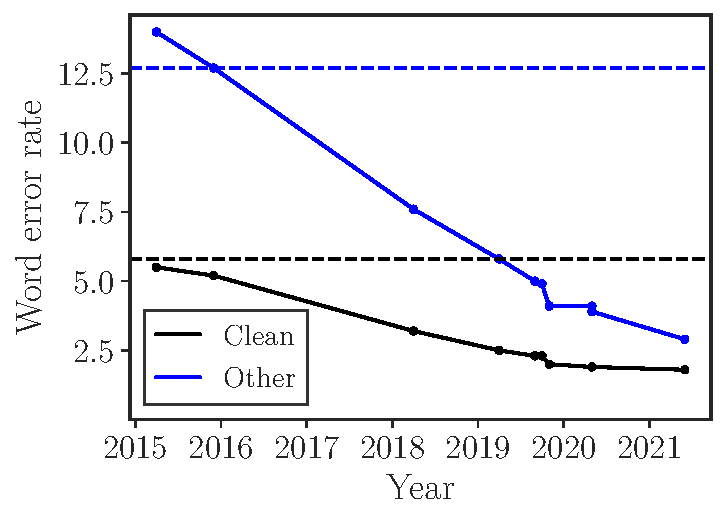
\includegraphics[width=\linewidth]{figures/librispeech_wer}
    \caption{LibriSpeech}
    \end{subfigure}
    \hfill
    \begin{subfigure}[b]{0.48\textwidth}
    \centering
    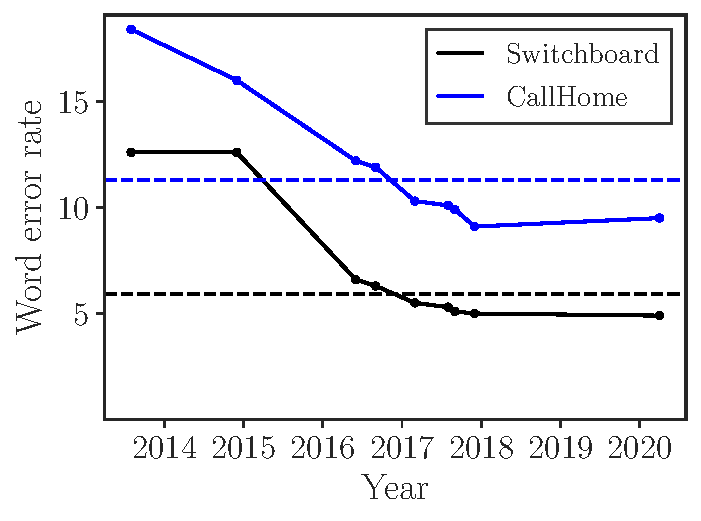
\includegraphics[width=\linewidth]{figures/switchboard_wer}
    \caption{Switchboard Hub5'00}
    \end{subfigure}
    \caption{The improvement in word error rate over time on the
    LibriSpeech~\citep{panayotov2015librispeech} and Switchboard Hub5'00
    benchmarks. The data for these figures is from
    \url{https://github.com/syhw/wer_are_we}. The dashed lines indicate
    human-level performance. The human-level results on LibriSpeech are
    reported in \citet{amodei2016deep} and those on Switchboard are reported in
    \citet{xiong2016achieving}.}
    \label{fig:wers}
\end{figure*}

\subsection{Word Error Rate}
\label{sec:wer}

{\bf Prediction:} By the end of the decade, possibly much sooner, researchers
will no longer be publishing papers which amount to "improved word error rate
on benchmark X with model architecture Y". As you can see in
figure~\ref{fig:wers}, word error rates on the two most commonly studied speech
recognition benchmarks have saturated.

Part of the problem is that we need harder benchmarks for researchers to
grapple with. The community has recently provided two new benchmarks that may
spur further research in speech recognition~\citep{chen2021gigaspeech,
galvez2021people}. However, I predict that these benchmarks will be quickly
saturated with the use of large neural networks and large scale
computation.

Another part of the problem is that we have reached a regime where word error
rate improvements on academic benchmarks no longer correlate with practical
value. Speech recognition word error rates on both benchmarks in
figure~\ref{fig:wers} surpassed human word error rates several years
ago.\footnote{Estimates of human-level word error rates on the CallHome portion
of Hub5'00 vary considerably. For example \citet{saon2017english} report a best
result 6.8 out of three transcribers whose results vary by nearly 2.0 absolute
word error rate.} On the other hand, in most settings humans are still better
than machines at understanding speech. This implies that word error rate as a
measure of the quality of a speech recognition system does not correlate well
with an ability to understand human speech.

A final issue is research in state-of-the-art speech recognition is becoming
less accessible as models are getting larger, data sets are getting larger, and
compute costs are increasing. A few well industry labs are rapidly becoming the
only places that can fund this type of research. As the advances become more
incremental and further from academia, this part of the field will continue to
shift from research labs to engineering organizations.

\subsection{Richer Representations}

{\bf Prediction:} Transcriptions will be replaced by richer representations for
downstream tasks which rely on the output of a speech recognizer. As mentioned
in section~\ref{sec:wer}, we have reached a regime on many academic benchmarks
in which word error rate no longer correlates with the true objective.

Downstream applications often don't care about a verbatim transcription; they
care about semantic correctness. Examples of downstream applications include
conversational agents, voice-based search queries, and digital assistants.

One possibility is to develop some sort of \emph{semantic error rate} and use
this to measure the quality of a speech recognizer. This is a challenging
albeit interesting research problem.

I think a much more likely outcome is to pass downstream applications richer
outputs from the speech recognizer. For example, instead of passing a single
transcription a lattice of possibilities which captures the uncertainty for
each could be much more useful.

{\bf Research implications:} The exact structure used to encode the
representation is an open question. One possibility could be some sort of
weighted transducer which if differentiable could allow for fine-tuning the
recognizer to specific applications~\cite{hannun2020differentiable, k2}. This
type of representation also requires models which are able to ingest variable
sized graphs as input.

\subsection{Personalization}

{\bf Prediction:} By the end of the decade, speech recognition models will be
deeply personalized to individual users. This is in part a direct
corollary of enabling on device training, but the motivation is distinct from
those discussed in section~\ref{sec:on_device}.

One of the main distinctions between the automatic recognition of speech and
the human interpretation of speech is in the use of context. Humans have much
more context available when listening to one another than. This context
includes the topic of conversation, what was said in the past, the noise
background, and visual cues like lip movement and facial expressions. I believe
we have, or will soon reach, the Bayes error rate for speech recognition on
short (\emph{i.e.} less than ten seconds) utterances taken out of context. Our
models are using the signal available in the data to the best of their ability.
To continue to improve the machine understanding of human speech will require
leveraging context as a deeper part of the recognition process.

One route for this is personalization. Personalization is already commonly used
to improve the recognition a given users contact list for utterances of the
form ``call \texttt{<NAME>}''. \citet{sim2019personalization} found
personalization to an individual users contacts improves named entity recall
from 2.4\% to 73.5\% -- a massive improvement. Personalizing models to
individual users with speech disorders improves word error rates by 64\%
relative~\citep{sim2019investigation}. Clearly personalization can make a huge
difference in the quality of the recognition, particularly for groups or
domains that are underrepresented in the training data. I predict we will see
much more pervasive personalization by the end of the decade.

{\bf Research implications:} Personalization requires on device training which
in itself requires lighter-weight models and likely some form of weak
supervision (see section~\ref{sec:on_device}). Furthermore, personalization
requires models which can be easily customized to a given user or context.
The best way to incorporate such context into a model is still a research
question.
